
\documentclass{article}
\usepackage{geometry} \geometry{margin=1in}
\usepackage{parskip}
\usepackage{ragged2e}
\usepackage{float}       % Required for [H]
\usepackage{tcolorbox}
\usepackage{amsmath, amssymb}
\usepackage{hyperref}     % Fixes "URL" errors
\usepackage{adjustbox}    % CRITICAL: Allows us to shrink huge diagrams
\usepackage{listings}     % For code blocks

% EXTENDED TIKZ LIBRARIES (Fixes "unknown library" errors)
\usepackage{tikz} 
\usetikzlibrary{shapes, arrows.meta, positioning, shadows, calc, fit, backgrounds, decorations.pathreplacing}

% GLOBAL STYLES
\tikzset{
    block/.style={rectangle, draw, thick, rounded corners, fill=blue!5, align=center, minimum height=2em},
    arrow/.style={thick, ->, >=stealth},
    decision/.style={diamond, draw, fill=green!10, align=center, aspect=2},
    cloud/.style={draw, ellipse, fill=red!10, node distance=3cm, minimum height=2em}
}
\raggedbottom

\begin{document}

% --- START OF CHUNK 1 ---

\section{Professionalism and the Conceptual Basis of Nursing}

\subsection{Distinguishing Profession from Occupation}

The foundation of nursing rests upon its establishment as a **profession**, a concept distinct from a simple **occupation**. While both involve work and contribute to society, the differences are significant. An occupation is often characterized by training that occurs on the job, with the length of training varying considerably. The work itself tends to be largely manual, and decision-making is frequently guided by experience or trial and error. Values, beliefs, and ethics are not necessarily central to preparation, and commitment and personal identification can be variable. Workers are often supervised, and job changes are common, with material reward serving as the primary motivation. Accountability typically rests with the employer.

In contrast, a profession requires education in a college or university, involving prolonged and rigorous study. The work demands mental creativity and is based on established science or theoretical constructs – what we now refer to as **evidence-based practice**. Values, beliefs, and ethics are integral to professional preparation, fostering a strong commitment and personal identification with the field. Professionals are autonomous, less likely to change professions, and motivated by a commitment that transcends material reward. Crucially, accountability rests with the individual practitioner. 

\begin{figure}[H]
    \centering
    \begin{adjustbox}{max width=\textwidth}
        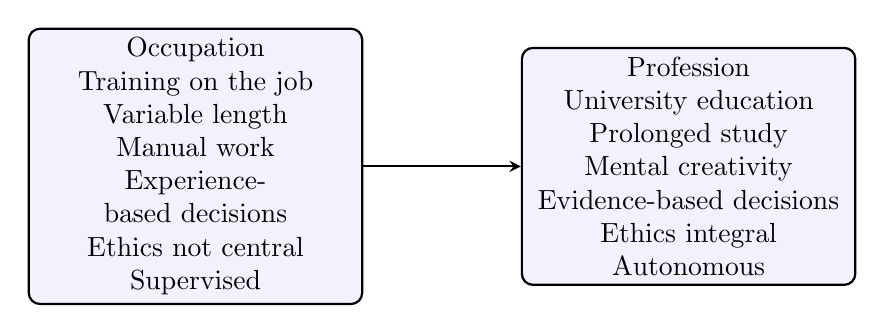
\begin{tikzpicture}[node distance=2cm, auto]
            \node[block, text width=4cm, align=center] (occupation) {Occupation\\Training on the job\\Variable length\\Manual work\\Experience-based decisions\\Ethics not central\\Supervised};
            \node[block, text width=4cm, align=center, right=of occupation] (profession) {Profession\\University education\\Prolonged study\\Mental creativity\\Evidence-based decisions\\Ethics integral\\Autonomous};
            \draw[arrow] (occupation) -- (profession);
        \end{tikzpicture}
    \end{adjustbox}
    \caption{Occupation vs. Profession}
\end{figure}

\subsection{Eight Characteristics of a Profession}

Kelly (1981) identified eight key characteristics that define a true profession. These characteristics are not merely aspirational; they represent the hallmarks of a field dedicated to serving humanity and upholding the highest standards of practice.

\textbf{Vital Service to Humanity:} The first characteristic emphasizes that the services provided by a profession are vital to humanity and the welfare of society. Nursing exemplifies this through its core focus on **caring**.  Many students are drawn to nursing precisely because of a desire to help others.  However, in today’s highly technological healthcare environment, it is crucial that nurses maintain the human aspects of caring, demonstrating empathy, compassion, and respect for patients’ dignity.  How nurses demonstrate caring is a constant reflection point in practice.

\textbf{Specialized Body of Knowledge:}  A profession possesses a unique and continually expanding body of knowledge acquired through research.  This is reflected in the growth of **research nursing degrees** and the increasing emphasis on **evidence-based practice**. Nursing relies on both theory and research to inform and guide clinical decision-making.

\textbf{Intellectual Activities and Accountability:}  Professional services involve intellectual activities, demanding critical thinking and problem-solving skills.  The **nursing process** itself – assessment, diagnosis, planning, implementation, and evaluation – is a prime example of this intellectual rigor.  Furthermore, a profession is defined by individual **accountability**. The American Nurses Association (ANA) defines accountability as being firmly rooted in ethical principles such as fidelity, loyalty, veracity, beneficence, and respect for patient autonomy.

\textbf{Education in Higher Learning:} Historically, nursing education has evolved towards institutions of higher learning. The University of Minnesota established the first university-based nursing program in 1909, followed by Yale in 1923.  The ANA formally advocated for all nursing education to take place in higher education institutions in 1965.  The ongoing debate regarding entry-level into practice highlights the importance of ensuring adequate preparation and a strong educational foundation.

\textbf{Autonomy and Control:}  Professionals are relatively independent and control their own policies and activities, a concept known as **autonomy**. This is supported by licensure and the ability to practice independently. While nurses often work under “doctor’s orders,” this connotation is evolving as the profession asserts its own expertise and scope of practice. Various groups influence nursing practice, including organized nursing, organized medicine, health service administration, and the Magnet Recognition Program.

\textbf{Altruism and Motivation:}  Professionals are motivated by a spirit of **altruism** – a selfless concern for the well-being of others. While nurses may seek fair compensation and improved working conditions, their fundamental motivation stems from a desire to serve.  **Collective bargaining** is one mechanism nurses use to advocate for both patient care and professional well-being.

\textbf{Code of Ethics:}  A profession operates under a clearly defined **code of ethics** to guide the decisions and conduct of its practitioners. The **Nightingale Pledge**, established in 1893, was an early expression of ethical commitment in nursing. Today, both the International Council of Nurses (ICN) and the ANA have established comprehensive Codes of Ethics that provide a framework for ethical decision-making in practice.

\begin{tcolorbox}[title=Definition]
\textbf{Value:} A deeply held belief or principle that guides behavior and influences decision-making.
\end{tcolorbox}

\begin{tcolorbox}[title=Definition]
\textbf{Belief:} A conviction or acceptance that something is true, even without absolute proof.
\end{tcolorbox}

\begin{tcolorbox}[title=Definition]
\textbf{Health:} A state of complete physical, mental, and social well-being, not merely the absence of disease or infirmity (WHO definition).
\end{tcolorbox}


% --- START OF CHUNK 2 ---

\section{Professionalism in Nursing}

\subsection{Characteristics of a Profession}

A true **profession** is characterized by a specific set of attributes that distinguish it from other occupations. One key characteristic, as highlighted, is the existence of an **organization** or **association** dedicated to promoting and upholding high standards of practice. In nursing, the **American Nurses Association (ANA)** serves as the official voice of the profession. The ANA advocates for nurses and the nursing profession, sets standards for nursing practice, and provides resources for professional development. However, despite the ANA's vital role, a relatively low percentage of nurses actually belong to the organization and its constituent state nurses associations. This limited membership can hinder the profession's collective voice and its ability to exert significant **political influence**.  A stronger, more unified nursing voice is crucial for shaping healthcare policy and ensuring that the needs of nurses and patients are adequately addressed.

\subsection{Barriers to Professionalism in Nursing}

Despite significant advancements, several barriers continue to impede the full realization of nursing as a profession. One major obstacle is the **varying levels of education** required for entry into practice. While a **Bachelor of Science in Nursing (BSN)** is increasingly recognized as the standard, nurses still enter the field with **Associate Degree in Nursing (ADN)** or **diploma** credentials. This lack of standardization impacts the depth and breadth of education, potentially affecting the quality of care and limiting opportunities for professional advancement.  David (2000) highlighted the need for a minimum BSN, and preferably an **Master of Science in Nursing (MSN)**, to fully prepare nurses for the complexities of modern healthcare.

Historically, **gender issues** have also played a role in shaping the perception and status of nursing.  Nursing has long been considered a "feminine" profession, which has sometimes led to undervaluation and limited opportunities for leadership.  Furthermore, **historic influences**, rooted in religious and military traditions, have historically emphasized obedience and service over independent thought and professional autonomy. 

**External conflicts**, particularly the traditional power dynamic between **medicine and nursing**, have also hindered nursing's professional development.  Historically, nursing has been positioned as subordinate to medicine, limiting nurses' authority and decision-making power. Finally, **internal conflicts** within the profession, such as **fragmented power and influence**, can weaken nursing's collective voice and impede progress toward professional goals.

\section{RN Education Programs}

\subsection{Types of Programs}

Nursing education pathways are diverse, catering to different career goals and educational backgrounds. These programs can be broadly categorized into **pre-licensure** and **post-licensure** programs. **Pre-licensure programs** are designed for individuals who do not yet hold a nursing license and aim to prepare them for initial licensure as a Registered Nurse (RN). These include:

*   **Diploma programs:** Historically significant, these programs were often hospital-based and have declined in number.
*   **Associate Degree in Nursing (ADN) programs:** These programs typically take two to three years to complete and focus on providing foundational nursing skills.
*   **Bachelor of Science in Nursing (BSN) programs:** Considered the gold standard, BSN programs are four to five-year programs that provide a broader education in nursing theory, research, and leadership.
*   **Graduate pre-licensure programs:** These accelerated programs allow individuals with a bachelor's degree in another field to earn a BSN.

**Post-licensure programs** are designed for RNs who wish to advance their education and skills. These include:

*   **RN to BSN programs:** Allow ADN or diploma-prepared nurses to earn a BSN.
*   **Advanced practice programs:** Lead to advanced practice registered nurse (APRN) roles, such as **Nurse Practitioner (NP)**, **Clinical Nurse Specialist (CNS)**, **Certified Nurse Midwife (CNM)**, and **Certified Registered Nurse Anesthetist (CRNA)**. These programs typically require a **Master of Science in Nursing (MSN)** or a **Doctor of Nursing Practice (DNP)** degree.
*   **Research degrees:** Such as a **PhD** or **Doctor of Science (DSc)**, prepare nurses for careers in nursing research and academia.

\subsection{Diploma Nursing Programs: A Historical Perspective}

**Diploma nursing programs** experienced a peak between 1920 and 1930, with approximately 200 programs operating in almost every state. However, these programs underwent a dramatic decline in the mid-20th century as nursing education increasingly shifted to institutions of higher education. Several factors contributed to this decline. The increasing **complexity of the healthcare environment** demanded a more comprehensive education than diploma programs could provide.  Furthermore, most **colleges and universities did not recognize diploma programs** for credit, limiting graduates' opportunities for further education.  While the number of diploma programs has significantly decreased, some programs still exist and have established **agreements with colleges and universities** to facilitate students' transition to BSN programs.  Historically, hospitals sometimes **misused these programs** by relying on student nurses as a source of inexpensive labor.

\subsection{Baccalaureate Programs: The Foundation of Professional Nursing}

**Baccalaureate programs (BSN)** are considered essential for qualifying nursing as a recognized profession and for preparing nurses for **leadership roles** in administration, teaching, and public health. The first BSN program was established in 1909 at the University of Minnesota, marking a pivotal moment in the professionalization of nursing. These programs typically span four to five years and include a combination of **general education requirements** and specialized **nursing courses**. BSN graduates are eligible to take the **NCLEX-RN** licensure exam and are well-prepared to pursue **graduate programs** and **advanced practice certification**. The **American Association of Colleges of Nursing (AACN)** published "The Essentials of Baccalaureate Education for Professional Nursing Practice" in 2008, outlining the core competencies and knowledge required of BSN graduates.

\subsection{Associate Degree Programs: A Focused Pathway}

**Associate Degree in Nursing (ADN)** programs were first introduced in 1952, based on a model developed by Mildred Montag. Montag's vision was to create a program that would prepare **nurse technicians** to provide routine care under the **supervision of professional nurses**. The ADN program was designed to be a shorter, more focused pathway to entry-level practice, primarily in **acute and long-term care settings**. It was intended to be an **end-point degree**, not necessarily a stepping stone to a BSN. However, contrary to the original intent, ADN graduates were later granted the right to sit for the **NCLEX-RN** examination, leading to increased enrollment in ADN programs.

\subsection{Articulated Programs: Facilitating Educational Mobility}

**Articulated programs** are designed to promote **mobility between programs**, allowing nurses to seamlessly advance their education. The **purpose** of these programs is to **facilitate opportunities** for nurses to move up the educational ladder. These programs often involve **multiple-entry and multiple-exit points**, allowing students to enter at different levels and exit with various credentials. **Articulation agreements** between institutions are crucial, as they **facilitate student movement** and **accept transfer credit**, resulting in **acceleration** or **advanced placement** within the nursing curriculum.

\subsection{RN to BSN and Graduate Entry Programs: Expanding Opportunities}

**RN to BSN programs** provide a pathway for nurses with an ADN or diploma to earn a BSN degree. These programs typically grant **credits** for prior nursing education and experience, allowing nurses to complete the BSN requirements more efficiently. They also often allow for the **transfer of general education courses** and offer **options for advanced placement**. **Graduate entry programs** offer an **accelerated or fast-track sequence** for individuals who already hold a bachelor's degree in another field to earn a second bachelor's degree in nursing, an **MSN (ELMS)**, or a **DNP**.


% --- START OF CHUNK 3 ---

\section{Advance Practice Degrees: Doctorate}

Doctoral programs are designed to prepare nurses for a variety of advanced roles, extending beyond direct patient care. These roles include positions as **faculty members** in universities, **administrators** within schools of nursing or large medical centers, **researchers** contributing to the evidence base of practice, **theorists** developing and refining nursing knowledge, and **advanced practitioners** providing specialized clinical care.  There are two primary types of doctoral degrees available to nurses: research-focused and practice-focused.

\subsection{Research-Focused Degrees}

A **research-focused degree** prepares nurses to generate new knowledge through rigorous investigation. The two main options in this category are the **Doctor of Philosophy (PhD)** and the **Doctor of Science (DSc)**. Both degrees emphasize research methodology, statistical analysis, and the dissemination of findings through publications and presentations.  The PhD is often considered the more traditional research degree, while the DSc may be more focused on applied research within a specific field of nursing.

\subsection{Practice-Focused Degrees}

The **Doctor of Nursing Practice (DNP)** is a **practice-focused degree** designed to prepare advanced practice nurses who will lead clinical practice change, translate research into practice, and improve patient outcomes.  Unlike the PhD, the DNP curriculum emphasizes clinical scholarship, evidence-based practice, and leadership skills.  The DNP is increasingly becoming the minimum requirement for advanced practice roles, reflecting a growing emphasis on the need for nurses with the highest level of clinical expertise and leadership capabilities.  This shift acknowledges that advanced practice requires not only a strong clinical foundation but also the ability to critically evaluate and implement research findings to optimize patient care.

\section{Systems Theory}

**Systems theory**, first articulated by **Ludwig von Bertalanffy** in 1936, provides a framework for understanding complex phenomena as interconnected wholes rather than isolated parts.  In nursing, this theory is invaluable for conceptualizing patients, healthcare organizations, and communities as **systems** with interacting components.  Understanding these interactions is crucial for effective assessment, intervention, and evaluation of care.

\subsection{Components of Systems}

All systems, regardless of their complexity, share several key components. These include:

\textbf{Input}: The resources, data, or energy that enter the system. In a healthcare context, this could be a patient's symptoms, a physician's order, or funding for a program.
\textbf{Throughput}: The processes that transform the input into output. This encompasses the actions taken within the system, such as nursing interventions, medical treatments, or administrative procedures.
\textbf{Output}: The results of the throughput process. This could be a patient's improved health status, a completed report, or a successful program implementation.
\textbf{Evaluation}: The assessment of the output to determine its effectiveness and identify areas for improvement.
\textbf{Feedback}: Information about the output that is used to adjust the input or throughput, creating a continuous cycle of improvement.

\section{Types of Systems}

Systems can be categorized based on their interactions with the external environment. The two primary classifications are **open systems** and **closed systems**.

\subsection{Open and Closed Systems}

An **open system** actively exchanges matter, energy, and information with its surroundings.  Most living systems, including individuals, families, and healthcare organizations, are open systems. This exchange allows them to adapt to changing conditions and maintain stability.  In contrast, a **closed system** does not interact with its environment.  While truly closed systems are rare in the real world, some systems may be relatively closed in certain respects. For example, a sealed laboratory experiment might be considered a closed system in terms of matter exchange.

\subsection{Subsystems and Supra-systems}

Within a larger system, smaller, interconnected units are known as **subsystems**.  For example, a hospital can be considered a system, and its various departments (e.g., cardiology, oncology) are subsystems. Conversely, a system exists within a broader context called a **supra-system**.  The healthcare system, for instance, is a subsystem of the larger societal system. Understanding these hierarchical relationships is essential for analyzing the influences that affect a system's functioning.

\section{Characteristics of Systems}

Systems exhibit several defining characteristics that contribute to their complexity and dynamic behavior.

\textbf{Holism}: The whole is different from and greater than the sum of its parts (its subsystems). This means that the interactions between components create emergent properties that cannot be predicted by examining the parts in isolation.
\textbf{Synergy}: Synergy occurs when the various subsystems work together to create a result that is not independently achievable.  Effective teamwork in healthcare exemplifies synergy, where the combined efforts of different professionals lead to better patient outcomes than could be achieved individually.
\textbf{Interdependence}: A change in one part of the system creates change in other parts. This highlights the interconnectedness of system components and the potential for ripple effects.
\textbf{Continuous Exchange}: There is continuous exchange of energy and information within open systems, between open systems, and with supra-systems. This exchange is vital for maintaining stability and adapting to change.
\textbf{Homeostasis}: Dynamic balance within and between subsystems, systems, and supra-systems helps create and maintain **homeostasis**, a state of internal stability.  The human body's ability to regulate temperature is a classic example of homeostasis.

\begin{figure}[H]
    \centering
    \begin{adjustbox}{max width=\textwidth}
        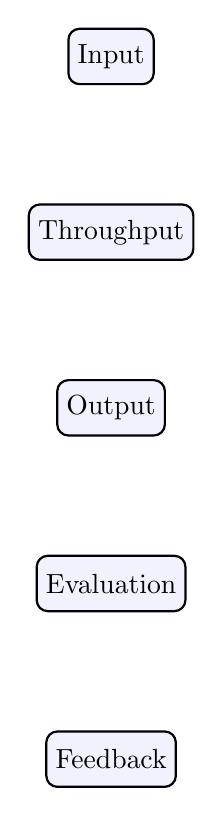
\begin{tikzpicture}[node distance=1.5cm, auto]
            \node[block, align=center] (input) {Input};
            \node[block, align=center, below=of input] (throughput) {Throughput};
            \node[block, align=center, below=of throughput] (output) {Output};
            \node[block, align=center, below=of output] (evaluation) {Evaluation};
            \node[block, align=center, below=of evaluation] (feedback) {Feedback};

            \path[arrow] (input) -- (throughput);
            \path[arrow] (throughput) -- (output);
            \path[arrow] (output) -- (evaluation);
            \path[arrow] (evaluation) -- (feedback);
            \path[arrow] (feedback) -- (input);
        \end{tikzpicture}
    \end{adjustbox}
    \caption{Basic System Model}
\end{figure}

\section{Key Concepts about Systems}

Several core concepts underpin the application of systems theory in nursing and healthcare.

A **system** is fundamentally a set of **interrelated parts**. These parts are not isolated entities but rather components that influence and are influenced by one another.
The parts collectively form a **meaningful whole**, possessing characteristics that transcend the sum of their individual components.
As previously emphasized, the **whole is different from and greater than the sum of its parts**.
**Systems may be open or closed**, depending on their degree of interaction with the external environment.
**All living systems are open systems**, constantly exchanging energy and information with their surroundings.
**Systems strive for homeostasis** (internal stability), maintaining a dynamic equilibrium despite external fluctuations.
**Systems are part of supra-systems**, existing within a broader context that influences their behavior.
**Systems have subsystems**, smaller units that contribute to the overall functioning of the system.
Finally, **a change in one part of a system creates change in other parts**, highlighting the interconnectedness and dynamic nature of systems.

\section{Fundamental Nursing Concepts}

Central to nursing practice are several fundamental concepts that provide a foundation for understanding the patient and the delivery of care.  One key concept is the **person**, viewed as an **open system with human needs**.

\subsection{The Person as a System}

In nursing, the **person** is considered an **individual** who is also an **open system** comprised of numerous **subsystems**. These subsystems include physiological, psychological, social, and spiritual dimensions, all interacting to maintain the individual's overall well-being. Each **person is unique**, shaped by their genetic makeup, environmental influences, and experiential history.

\subsection{Human Needs and Maslow's Hierarchy}

**Human needs** are essential for a person's well-being and are often categorized using frameworks like **Maslow's Hierarchy of Needs**.  **Abraham Maslow** (1954) proposed that human behavior is motivated by intrinsic needs, arranged in a hierarchical order. He identified five levels of needs: physiological, safety, love/belonging, esteem, and self-actualization.  These needs must be met in a sequential manner, with lower-level needs taking precedence over higher-level needs.

\begin{figure}[H]
    \centering
    \begin{adjustbox}{max width=\textwidth}
        \includegraphics[width=\textwidth]{maslow.png}
    \end{adjustbox}
    \caption{Maslow's Hierarchy of Needs}
\end{figure}

\subsection{Assumptions About Maslow's Hierarchy}

Several key assumptions underlie Maslow's Hierarchy. First, **basic needs must be at least partially satisfied before higher-order needs can become relevant to the individual**.  A person struggling with hunger or lack of shelter will likely prioritize those needs over social connection or self-esteem. Second, **individuals meet their needs in different ways**, reflecting their unique values, beliefs, and cultural backgrounds.  Finally, **the manner in which needs are met and the extent to which they are considered important vary according to each individual**. This underscores the importance of **individualized nursing care**, tailoring interventions to address the specific needs and priorities of each patient.


% --- START OF CHUNK 4 ---

\section{Adaptation and Human Needs}

\subsection{Carl Rogers and the Changing Self}

The work of **Carl Rogers** (1961) in *On Becoming a Person* highlights a fundamental principle of human experience: a person’s **needs** are not static, but rather evolve alongside the individual’s growth and change. This perspective moves away from a hierarchical view of needs, where certain deficiencies must be met before others can be addressed. Instead, it emphasizes the dynamic interplay between the self and the environment, where needs emerge from the ongoing process of becoming.  Understanding this fluidity is crucial in nursing, as patient needs are rarely fixed and require continuous assessment and adaptation of care plans.

\subsection{The Concept of Adaptation}

**Adaptation** refers to the process by which individuals adjust to changes in their environment.  This adjustment isn't merely about survival; it's about maintaining a sense of well-being and psychological equilibrium. A clear example of the challenges of adaptation is observed in patients admitted to hospitals.  Removal from their familiar surroundings, routines, and social support systems often leads to **anxiety**. This demonstrates the profound impact of the environment on an individual’s psychological state and underscores the importance of creating a supportive and therapeutic hospital environment.  The disruption of established patterns necessitates a period of readjustment, and nurses play a vital role in facilitating this process.

\section{Homeostasis}

\subsection{Dynamic Balance and Open Systems}

**Homeostasis** is a central concept in understanding physiological and psychological health. It describes the dynamic balance achieved by effectively functioning **open systems**. Unlike closed systems, open systems interact with their environment, exchanging matter and energy.  In the context of the human body, homeostasis is maintained through coordinated responses of organ systems that automatically compensate for environmental changes. For example, the body regulates temperature, blood pressure, and fluid balance to maintain a stable internal environment despite external fluctuations.

\subsection{Individual and Environmental Balance}

Individuals, as open systems, also strive to maintain balance between **external and internal forces**. This extends beyond purely physiological regulation to encompass psychological and social well-being. When this balance is achieved, the person is considered healthy or possesses resistance to illness. However, if **adaptation** is unsuccessful, **disequilibrium** can occur, creating a vulnerability to the development of illness or disease.  This highlights the interconnectedness of physical, psychological, and environmental factors in health and illness.

\section{Fundamental Nursing Concepts}

\subsection{The Environment as a Supra-System}

In nursing, the **environment** is conceptualized as a **supra-system** – the overarching context in which a person lives. This system encompasses not only the physical surroundings but also the social, cultural, and economic factors that influence health and well-being. The environment is not a neutral backdrop; it can actively **promote or interfere with homeostasis** and the overall well-being of individuals.

\subsection{Maslow's Hierarchy and Environmental Influence}

**Maslow’s hierarchy of needs** provides a framework for understanding the dynamic interaction between a person’s internal needs and the external environment.  The satisfaction of these needs – physiological, safety, love/belonging, esteem, and self-actualization – is often dependent on environmental factors. For instance, access to adequate food, shelter, and healthcare (physiological and safety needs) are directly influenced by socioeconomic conditions and healthcare systems.  Nurses must consider these environmental determinants of health when assessing and addressing patient needs.

\section{Environmental Systems}

\subsection{Levels of Environmental Influence}

Environmental systems operate at multiple levels, each influencing individual health in unique ways. These include:

*   **Family systems:** The immediate social unit providing support, socialization, and emotional connection.
*   **Cultural systems:** Shared beliefs, values, and practices that shape health behaviors and perceptions of illness.
*   **Social systems:** Encompassing **communities**, **states**, **nations**, **supra-national** organizations, and the **international** community. Each level exerts influence on health policies, resource allocation, and access to care.

\subsection{The Nurse's Environmental Impact}

Nurses have a significant **potential impact on the environment/supra-system** through their practice and advocacy. This includes promoting **ecological health** by minimizing environmental hazards, creating **healthy work environments** for themselves and colleagues, and participating in initiatives such as **WHO training modules** on issues like **mercury poisoning**.  Organizations like **Health Care Without Harm** are dedicated to reducing hazardous waste in healthcare settings, demonstrating a commitment to environmental sustainability. The **Luminary Project** exemplifies efforts to improve healthcare practices through environmental stewardship.

\section{Fundamental Nursing Concepts}

\subsection{Health as a Continuum}

The concept of **health** is often viewed as a **continuum**, rather than a fixed state. This means that health is not simply the absence of disease, but rather a dynamic process of striving for optimal well-being.  **Definitions of health vary** depending on individual perspectives, cultural beliefs, and theoretical frameworks.

\subsection{Health Beliefs and Locus of Control}

Several **health beliefs models** attempt to explain how individuals perceive and respond to health risks. These include:

*   **Rosenstock’s Health Beliefs Model:**  Focuses on an individual’s perception of susceptibility, severity, benefits, and barriers to taking action.
*   **Bandura’s Theory of Self-Efficacy:**  Emphasizes the belief in one’s ability to successfully execute a behavior.

Furthermore, an individual’s **locus of control** – their belief about the source of control over their life – influences their health behaviors.  An **internal locus of control** suggests that individuals believe they have control over their own health outcomes, while an **external locus of control** attributes outcomes to external factors such as fate or luck.

\begin{figure}[H]
    \centering
    \begin{adjustbox}{max width=\textwidth}
        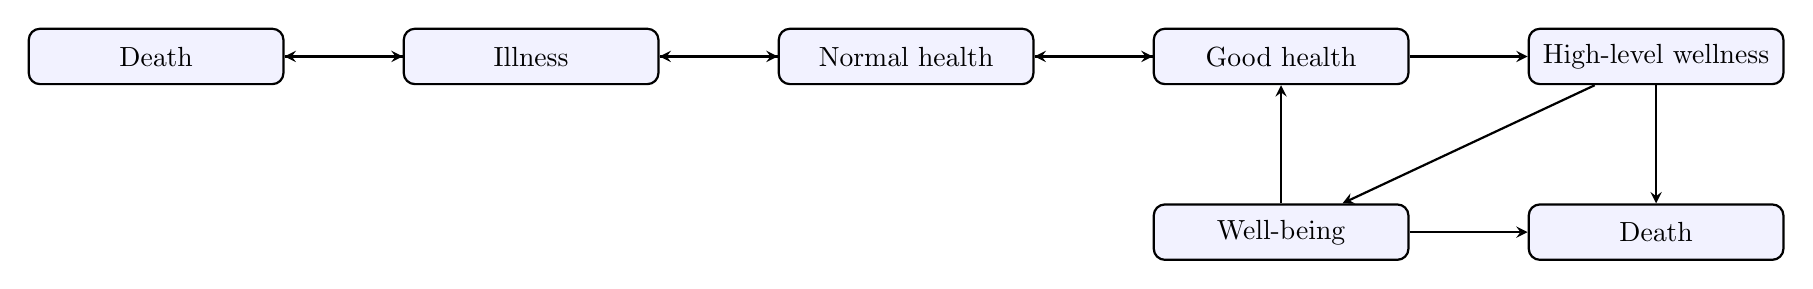
\begin{tikzpicture}[node distance=1.5cm, auto]
            \node[block, text width=3cm, align=center] (death_left) {Death};
            \node[block, text width=3cm, align=center] (illness) [right=of death_left] {Illness};
            \node[block, text width=3cm, align=center] (normal_health) [right=of illness] {Normal health};
            \node[block, text width=3cm, align=center] (good_health) [right=of normal_health] {Good health};
            \node[block, text width=3cm, align=center] (high_wellness) [right=of good_health] {High-level wellness};
            \node[block, text width=3cm, align=center] (death_right) [below=of high_wellness] {Death};
            \node[block, text width=3cm, align=center] (wellbeing) [below=of good_health] {Well-being};

            \draw[arrow] (death_left) -- (illness);
            \draw[arrow] (illness) -- (normal_health);
            \draw[arrow] (normal_health) -- (good_health);
            \draw[arrow] (good_health) -- (high_wellness);
            \draw[arrow] (high_wellness) -- (wellbeing);
            \draw[arrow] (wellbeing) -- (good_health);
            \draw[arrow] (good_health) -- (normal_health);
            \draw[arrow] (normal_health) -- (illness);
            \draw[arrow] (illness) -- (death_left);
            \draw[arrow] (high_wellness) -- (death_right);
            \draw[arrow] (wellbeing) -- (death_right);
        \end{tikzpicture}
    \end{adjustbox}
    \caption{Health as a Continuum}
\end{figure}

\section{Nursing: Forming the Meaningful Whole}

\subsection{Holistic Nursing Care}

**Holistic nursing care** nourishes the **whole person** – encompassing the **body, mind, and spirit**. This approach recognizes the interconnectedness of these dimensions and seeks to address the individual’s unique needs in a comprehensive manner. Eight factors contribute to a holistic approach to nursing:

1.  Nursing is an **open system**, constantly interacting with and influenced by the environment.
2.  Nursing is the **provision of health care services**, encompassing a wide range of interventions.
3.  Nursing **involves collaborating with patients and their families**, recognizing their expertise and preferences.
4.  Nursing is **integrally involved with people**, focusing on their individual experiences and values.
5.  Nursing care is provided **regardless of diagnosis, individual differences, age, beliefs, gender, sexual orientation, or other factors**, ensuring equitable and compassionate care.
6.  Nurses **require advanced knowledge and skills** to effectively address complex patient needs.
7.  Nursing requires **concern, compassion, respect, and warmth**, as well as comprehensive, individualized planning of care, to facilitate patients’ growth toward wellness.
8.  Nursing **links theory and research**, ensuring that practice is evidence-based and continually evolving.

\section{Beliefs Guiding Nursing Behaviors}

\subsection{Understanding Belief Systems}

**Beliefs** are fundamental to understanding human behavior and are central to nursing practice. They can be defined as **what people believe to be true**, influencing their **attitudes and behaviors**. **Belief systems** serve to guide **thinking and decision-making**, providing a framework for interpreting the world and making choices.

\subsection{Types of Beliefs}

Beliefs can be categorized into several types:

*   **Descriptive or existential beliefs:**  Concerns about the nature of reality and the meaning of life.
*   **Evaluative beliefs:**  Judgments about the goodness or badness, rightness or wrongness of things.
*   **Prescriptive (encouraged) and proscriptive (prohibited) beliefs:**  Rules and norms that dictate what behaviors are acceptable or unacceptable.

Understanding a patient’s belief system is crucial for providing culturally sensitive and effective care.

\section{Values}

\subsection{Defining Values}

**Values** are **freely chosen principles, ideals, or standards** held by an individual, class, or group that give **meaning and direction to life**. They represent an **abstract representation of what is right, worthwhile, or desirable**. Importantly, values are relatively **stable and resistant to change**, forming a core part of an individual’s identity.

\subsection{The Valuing Process}

The process of valuing involves three key steps:

1.  **Choosing:** The **cognitive (intellectual) aspect** of valuing, involving a deliberate selection of beliefs and principles.
2.  **Prizing:** The **affective (emotional) aspect** of valuing, where chosen beliefs are imbued with emotional significance.
3.  **Acting:** The **kinesthetic (behavioral) aspect** of valuing, where beliefs are translated into consistent actions.

It is essential that **all three steps are taken** for the process of valuing to be complete.  A value that is intellectually acknowledged but not emotionally embraced or consistently acted upon is unlikely to guide behavior effectively.


% --- START OF CHUNK 5 ---
\section{Values Clarification}

\subsection{Identifying Nursing Values}

Nursing is a profession deeply rooted in **ethics** and **values**. These values guide our practice, influence our decision-making, and shape the care we provide to patients. However, values are personal and can vary significantly between individuals. This can lead to moral dilemmas, especially in complex healthcare situations.  A crucial step in professional development is **values clarification** – a process of identifying, examining, and prioritizing one's own beliefs and values. This process is not about finding "right" or "wrong" answers, but rather about understanding *why* you hold certain beliefs and how those beliefs will impact your nursing practice.  The following statements are designed to prompt reflection on your own values and how they align with the core principles of nursing.

Consider the statement: “Patients should always be told the truth about their diagnoses.”  This touches upon the principles of **autonomy** and **beneficence**.  Patients have the right to make informed decisions about their healthcare, and that requires full disclosure of relevant information. However, there are cultural considerations and potential psychological impacts to consider.  Some believe a more gradual or filtered approach to truth-telling is more compassionate.  Where do you fall on this spectrum, and why?

The statement, “Nurses, if asked, should assist terminally ill patients to die,” is particularly challenging. This directly relates to the complex and often controversial topic of **assisted suicide** or **physician-assisted death**.  Nursing’s traditional role is to preserve life, but increasingly, nurses are encountering patients who desire control over their dying process.  Legal and ethical frameworks surrounding this issue vary widely, and nurses must be aware of the laws in their jurisdiction and their own organizational policies.  Your personal beliefs about the sanctity of life, patient autonomy, and the role of suffering will heavily influence your response to this statement.

Next, consider: “Severely impaired infants should be kept alive, regardless of their future quality of life.” This statement raises profound ethical questions about **infanticide**, **quality of life**, and the limits of medical intervention.  It forces us to confront difficult questions about what constitutes a “life worth living” and who has the right to make that determination.  This is often a deeply emotional issue, and personal beliefs about disability, suffering, and parental rights play a significant role.

The statement “Nurses should never accept gifts from patients” addresses the issue of **professional boundaries** and **potential conflicts of interest**. While a small token of gratitude may seem harmless, accepting gifts can blur the lines between a professional relationship and a personal one. It can also create an expectation of preferential treatment or compromise objectivity in care.  Many healthcare organizations have strict policies prohibiting or limiting gift acceptance.

The statement, “A college professor should receive a heart transplant before a homeless person does,” highlights the complex issue of **resource allocation** in healthcare.  In a world of limited resources, difficult decisions must be made about who receives life-saving treatments.  This statement forces us to confront our biases and consider the principles of **justice** and **equity**.  Should access to healthcare be based on social status, contribution to society, or simply medical need?

Finally, “Nurses should be role models of healthy behavior” emphasizes the importance of **professionalism** and **integrity**.  Nurses are often seen as trusted sources of health information, and their actions can have a significant impact on the health behaviors of others.  This includes not only promoting healthy lifestyles but also practicing what we preach – maintaining our own physical and mental well-being.





\end{document}